\section{Experiential Learning Activities}

This project will address the the needs of community college students and the AI workforce through open source micro-internships as experiential learning.

Internships are one of the most important forms of experiential learning students can undertake. They help students learn to deal with resistance and teammates, do research, manage their time, make sound decisions, and gain confidence in their abilities.\cite{beaubouefComputerScienceCurriculum2011} From the point of view of a student, internships make the biggest impact on how likely they are to be hired,\cite{callananAssessingRoleInternships2004,jonesTransformingCurriculumPreparing2002,knouseRelationCollegeInternships1999,saltikoffPositiveImplicationsInternships2017,stepanovaHiringCSGraduates2021} as well as being a deciding factor when competing for others for a job.\cite{grayInternshipExperienceMost} From the point of view of employers, internships help students understand how to apply what they have learned.\cite{beaubouefComputerScienceCurriculum2011}

\subsection{Addressing Time, Skill, and Knowledge Barriers with Micro-Internships}

CTC students face several practical barriers to participating in traditional internships:

\begin{enumerate}
    \item Many CTC students may not have completed enough coursework to meaningfully participate in a traditional internship.
    \item Many CTC students are unable to commit the time necessary to participate in an internship. 34\% of 4-year university students cited time conflicts with higher life priorities as the reason for not securing an internship in a 2020 study.\cite{kapoorBarriersSecuringIndustry2020} This number is likely even higher for CTC students, who are more likely to have caregiving responsibilities for family members and rely on a job for year-round financial support.\cite{AlmanacAmericanEducation,phillippeNationalProfileCommunity2005}
\end{enumerate}

To address these barriers, this project will use micro-internships. These are internships with a shorter timeframe (under 40 hours of work) and a simplified task.\cite{wingardWhyMicroInternshipsWill} Like traditional internships, micro-internships are a form of work-based, experiential learning where students perform relevant and meaningful tasks under the guidance of a mentor, with a focus on training and feedback.\cite{PowerWorkBasedLearning} CodeDay will create these micro-internships working on open source AI projects under the guidance of AI industry mentors.

Students who participate in micro-internships receive many of the same benefits as traditional internships: more knowledge and experience, improved confidence to pursue a degree, and an increased enjoyment of their degree.\cite{menezesWhatSkillsCS2023} Companies have also become interested in micro-internships as a way to build skills, get early access to talent, and support diversity and inclusion.\cite{mossMicroInternshipsPowerfulTool2019}

\subsection{Developing the Knowledge, Skills, and Proficiency in AI Through Micro-Internships}

In a paper accepted for publication at IEEE Frontiers in Education in October 2023, CodeDay partnered with California State University, Monterey Bay to offer micro-internships for 175 students attending CTCs and state colleges, and found that the format proposed for this project can be successful for general Computer Science students.\cite{narayananScalableApproachSupport2023} In that group, 90\% of students completed a micro-internship by successfully contributing to an open-source project. The proposed project will adapt this successful model for the emerging technology of AI, and offer it exclusively to CTC students.

\textit{Can an early-stage micro-internship meaningfully build knowledge and skills that CTC students need for an AI career?} When considering recent computer science graduates, employers report that they are unconcerned with the level of specific technical knowledge of today's graduates but find that graduates are lacking in the ability to work independently without step-by-step direction (the ``core software engineering process'') and soft skills.\cite{menezesWhatSkillsCS2023} Micro-internships help students start to build these skills. A majority of students who completed micro-internships as part of the aforementioned study continued to make contributions to open source software, where they likely gained additional skills. Overall, students were nearly twice as likely to get a traditional internship or job as compared to their peers. This responds to the ExLENT program’s criterion that the project must develop the interests, motivations, skills, knowledge, and/or proficiencies of workers in emerging technology.

\subsection{Micro-Internship Format}

In order to participate in micro-internships, students will need to meet baseline knowledge requirements by taking classes in their school: a demonstrated knowledge of functions, classes, and variables, and the ability to design and run a CS101-level application; the ability to read and understand code written by others; at least some experience doing independent research to solve a problem; and basic knowledge of collaboration tools such as Git.

Each student will participate in at least one, and up to two micro-internships in each cohort. Two opportunities will be available in the fall, and an additional three opportunities will be available in the winter/spring. (See Figure \ref{fig:cohortCalendar}.) Most students who register to participate in this project are expected to be eligible by the November deadline for session 2. All additional prerequisites will be provided during the onboarding week.

\subsubsection{Mentor/Project Recruiting and Matchmaking}

\begin{wrapfigure}{r}{0.25\textwidth} %this figure will be at the right
    \centering
    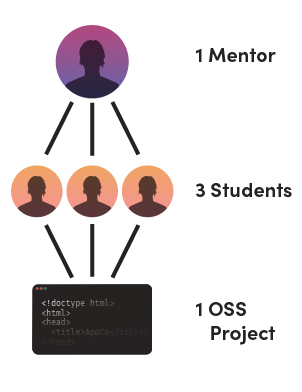
\includegraphics[width=0.25\textwidth]{oss}
\end{wrapfigure}

Mentors with experience in AI will be recruited from the employer constituents of project collaborator WTIA (see ``Partnerships''), from advertising on LinkedIn, and through CodeDay and MinT's existing pool of mentors (see ``Facilities, Equipment, and Other Resources'').

During the micro-internship, students will make contributions to an assigned task in an AI-focused open source project. Open source projects are collaborative initiatives in which an application's source code is made freely available online, and maintainers invite contributions from a global community of volunteers. CodeDay has already built partnerships with many AI open source projects for its summer internship program\cite{menezesOpenSourceInternshipsIndustry} and will select student tasks from the pool collected for that purpose. (See ``Facilities, Equipment, and Other Resources''.) Students will be grouped into teams of 2-3 students + 1 mentor based on availability, and projects will be assigned at random.

Tasks selected for the micro-internship, while a meaningful first introduction to contributing to an AI project, are expected to be very simple. An experienced developer could solve each selected task in under one hour.

Mentors are not expected to have any experience with the project they are assigned. An important feature of the micro-internship design is for mentors to act as a near-peer with regard to the selected issue and to model learning behavior, rather than acting like an instructor who knows the answers.

\subsubsection{Onboarding}

The first week of each micro-internship will prepare students to work on their project. Students will complete educational modules to learn about contributing to open-source software, and then begin preparing for their first mentor meeting. This content has already been created (see ``Facilities, Equipment, and Other Resources''). However, a module to better prepare students for AI projects is anticipated in response to student feedback:

\begin{enumerate}
    \item \textit{Introduction to Open Source:} Describe what it means for something to be open source and how it's used to collaborate on software; use Git to commit and push code changes; open a Pull Request.
    \item \textit{Introduction to AI/ML:} [Module will be created in this project, but is expected to result in: explain how and why data is split into training and test data; describe the basic ideas behind machine learning without requiring math; define common terms used in AI/ML codebases.]
    \item \textit{Software Engineering Process:} Read an unfamiliar line of code and create a written brainstorm of what it may do; read an unfamiliar class or file and brainstorm the purpose of the class; create a codebase diagram tracing which files may be related to an assigned task; identify potential ``starting points'' in a codebase for an issue.
    \item \textit{Collaboration:} Identify the difference between building in development and installing a project; conduct a pair programming meeting.
\end{enumerate}

After completing education modules, students will fill out a template to learn about their project and prepare for their mentor meeting. In the first mentor meeting, the mentor will review the students' answers:

\begin{itemize}
    \item Explain what the project does in your own words.
    \item Explain what the issue you've been assigned is asking you to do in your own words.
    \item Identify two ways to get support from the maintainers or the community.
    \item Identify three written documentation sources or support resources provided by the project which may be helpful in your issue.
    \item Identify two frameworks that seem important for the project.
    \item Identify three potential ``starting points'' for your work on the issue.
    \item List at least one specific question you have for your mentor.
\end{itemize}

\subsubsection{Project Work}

In weeks 2-4, student teams will collaborate using synchronous calls, synchronous in-person meetings, asynchronous chat programs, issue tracking software, and online code reviews. Each team's assigned mentor will meet with the team virtually in one 90-minute meeting each week. The agenda for the first meeting will be driven by the student agendas submitted in ``Mentor Meeting Preparation'' on the LMS, while the following two meetings will be driven directly by student questions. Students can book time with CodeDay's TAs, a team of more advanced students who are available to provide assistance with identifying and debugging code (see ``Facilities, Equipment, and Other Resources'').

Students will provide twice-weekly updates, and mentors will provide feedback each week and at the end of the program. (See ``Evaluation''.)

\subsubsection{Project Reflection}

Students will complete a project reflection in the form of a blog post and/or a 10 minute technical talk video, which can be shared with potential employers. The reflection will include a background of the project and the assigned issue, high-level overview of the relevant parts of the codebase, description of the changes the student made, and lessons learned.